\section{Kapitel 1}
Codebeispiel in \autoref{code:useEffect-sample}

\codefull{code:useEffect-sample}{Implementierung des \codeinline{useEffect}-Hooks}{jsx}{code/useEffect-sample.jsx}

% Mit extra optionen
\codefull[firstline=4, lastline=6]{code:useEffect-sample-options}{Implementierung des \codeinline{useEffect}-Hooks}{jsx}{code/useEffect-sample.jsx}

Abbildung in \autoref{img:redux-saga-flow}

\begin{figure}[H]
	\centering
	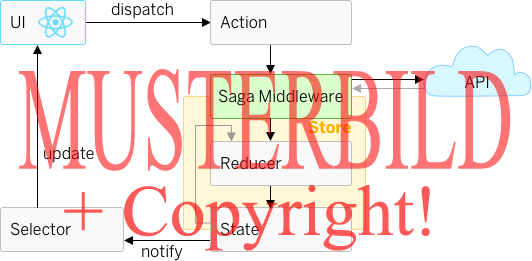
\includegraphics[height=6cm]{redux-saga-flow}
	\caption{Datenfluss mit Redux und Redux-Saga als Bibliothek}
	\label{img:redux-saga-flow}
\end{figure}

Abbildungen nebeneinander mit Frame in \autoref{img:tabl}

\begin{figure}[H]
	\centering
	\begin{subfigure}[b]{.45\textwidth}
		\centering
		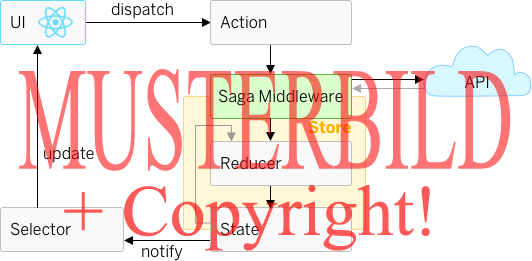
\includegraphics[width=1.0\textwidth, cframe=imageFrameGray]{redux-saga-flow}
		\caption{Kopfleiste}
		\label{img:tablet-head}
	\end{subfigure}
	\begin{subfigure}[b]{.45\textwidth}
		\centering
		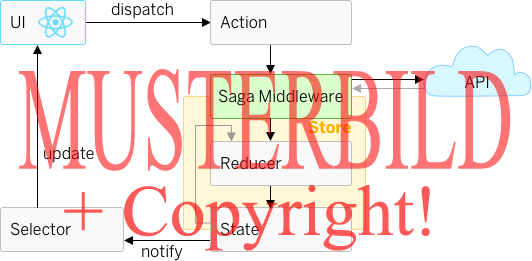
\includegraphics[width=1.0\textwidth, cframe=imageFrameGray]{redux-saga-flow}
		\caption{Filtermenü}
		\label{img:tablet}
	\end{subfigure}
	\caption{Vorführmodell des Statistikfilters für Tabletgeräte}
	\label{img:tabl}
\end{figure}

Tabelle in \autoref{tab:sec-verification-runs}

\begin{longtable}[c]{p{1cm} p{9cm} p{4cm}} 
	\hiderowcolors
	\caption{Ablauf und Ergebnis der Testszenarien für die Sicherheitsanforderung}
	\label{tab:sec-verification-runs}\\
	\bottomrule
	\showrowcolors
	\rowcolor{tableHeadColor}
	\textbf{ID} & \textbf{Ablauf} & \textbf{Ergebnis} \\
	%\midrule
	\hline
	\endfirsthead
	%
	\hiderowcolors
	\multicolumn{3}{c}{{\textit{Tabelle \thetable\ von letzter Seite fortgesetzt} }} \\
	\endhead
	%
	%\hline
	\multicolumn{3}{r}{\textit{Fortsetzung auf nächster Seite}} \\
	\endfoot
	%\hline
	\endlastfoot
	\showrowcolors
	%
	TS1 &
	\begin{minipage}[t]{9cm}
		\begin{enumerate}
			\item Testnutzer erhält Rolle für sein Profil
			\item Testnutzer meldet sich im Netzwerk mit seinem Profil an
			\item Testnutzer ruft Webanwendung auf
		\end{enumerate}
	\end{minipage}  & 
	\begin{minipage}[t]{4cm}
		\textcolor{applegreen}{$ \checkmark $ } bestanden
	\end{minipage}  \\ 
	TS2 &
	\begin{minipage}[t]{9cm}
		\begin{enumerate}
			\item Testnutzer meldet sich im Netzwerk mit seinem Profil an
			\item Testnutzer ruft Webanwendung auf
		\end{enumerate}
	\end{minipage}  & 
	\begin{minipage}[t]{4cm}
		\textcolor{applegreen}{$ \checkmark $ } bestanden
	\end{minipage}  \\ 
	TS3 &
	\begin{minipage}[t]{9cm}
		\begin{enumerate}
			\item Testnutzer erhält Rolle für sein Profil
			\item Testnutzer ruft Webanwendung auf
		\end{enumerate}
	\end{minipage}  & 
	\begin{minipage}[t]{4cm}
		\textcolor{applegreen}{$ \checkmark $ } bestanden
	\end{minipage}  \\ 
	TS4 &
	\begin{minipage}[t]{9cm}
		\begin{enumerate}
			\item Testnutzer erhält Rolle für sein Profil
			\item Testnutzer meldet sich im Netzwerk mit seinem Profil an
			\item Testnutzer wartet bis Sitzung nicht mehr gültig ist
			\item Testnutzer besucht Webanwendung
		\end{enumerate}
	\end{minipage}  & 
	\begin{minipage}[t]{4cm}
		\textcolor{applegreen}{$ \checkmark $ } bestanden
	\end{minipage}  \\ 
	TS5 &
	\begin{minipage}[t]{9cm}
		Alle Schritte aus TS4 werden durchlaufen und folgende Schritte werden danach ausgeführt:
		\begin{enumerate}
			\item Sitzung wird invalidiert/deaktiviert (entweder durch Entfernen des Sitzungstoken-Cookies, oder durch Ablaufen der Sitzung)
			\item Testnutzer lädt neue Statistiken
		\end{enumerate}
	\end{minipage}  & 
	\begin{minipage}[t]{4cm}
		\textcolor{applegreen}{$ \checkmark $ } bestanden
	\end{minipage}  \\
	\bottomrule     
\end{longtable}

Refernz auf \cite{augsten_2017_was}.